\documentclass[tikz,border=10pt]{standalone}
% Shared preamble for the CenterTask panel files (panel_a/b/c.tex).
% Edit colours and node styles here, once.
\usepackage{amsmath}
\usetikzlibrary{arrows.meta,positioning,calc}

% category colours as in ColorCategoryMap.m: 1=Short/Orange, 2=Mid/Green, 3=Long/Blue
\definecolor{catShort}{RGB}{243,178,132}
\definecolor{catMid}{RGB}{158,209,172}
\definecolor{catLong}{RGB}{157,188,234}

\tikzset{ctpanel/.style={
  font=\sffamily,
  band/.style={rounded corners=6pt, fill=black!7, draw=none, inner sep=8pt, minimum height=1.15cm},
  unit/.style={circle, fill=catMid!60, draw=none, minimum size=0.95cm, inner sep=0pt},
  flow/.style={-{Latex[length=2.2mm]}, line width=0.8pt},
  rowlab/.style={anchor=east, font=\sffamily\large},
  now/.style={fill=catShort!55, rounded corners=3pt, inner sep=3pt},
  stage/.style={rounded corners=6pt, fill=black!8, draw=none, inner sep=8pt, minimum height=1.2cm, align=center},
  target/.style={circle, minimum size=0.9cm, inner sep=0pt, draw=none, font=\sffamily\scriptsize, text=black!75},
  axis/.style={line width=0.6pt},
}}


% ---------------------------------------------------------------------
%  Many-to-many, unrolled: what x_t and y_t are for each of the three
%  networks, and how it differs from many-to-one.
%  Row 1: trial-level tiny RNN   (one step = one trial, sequence = session)
%  Row 2: within-trial task RNN  (one step = 10 ms, sequence = one trial)
%  Row 3: motor GRU              (one step = 10 ms, sequence = one trial)
%  Right: many-to-one vs many-to-many topologies.
% ---------------------------------------------------------------------

\begin{document}
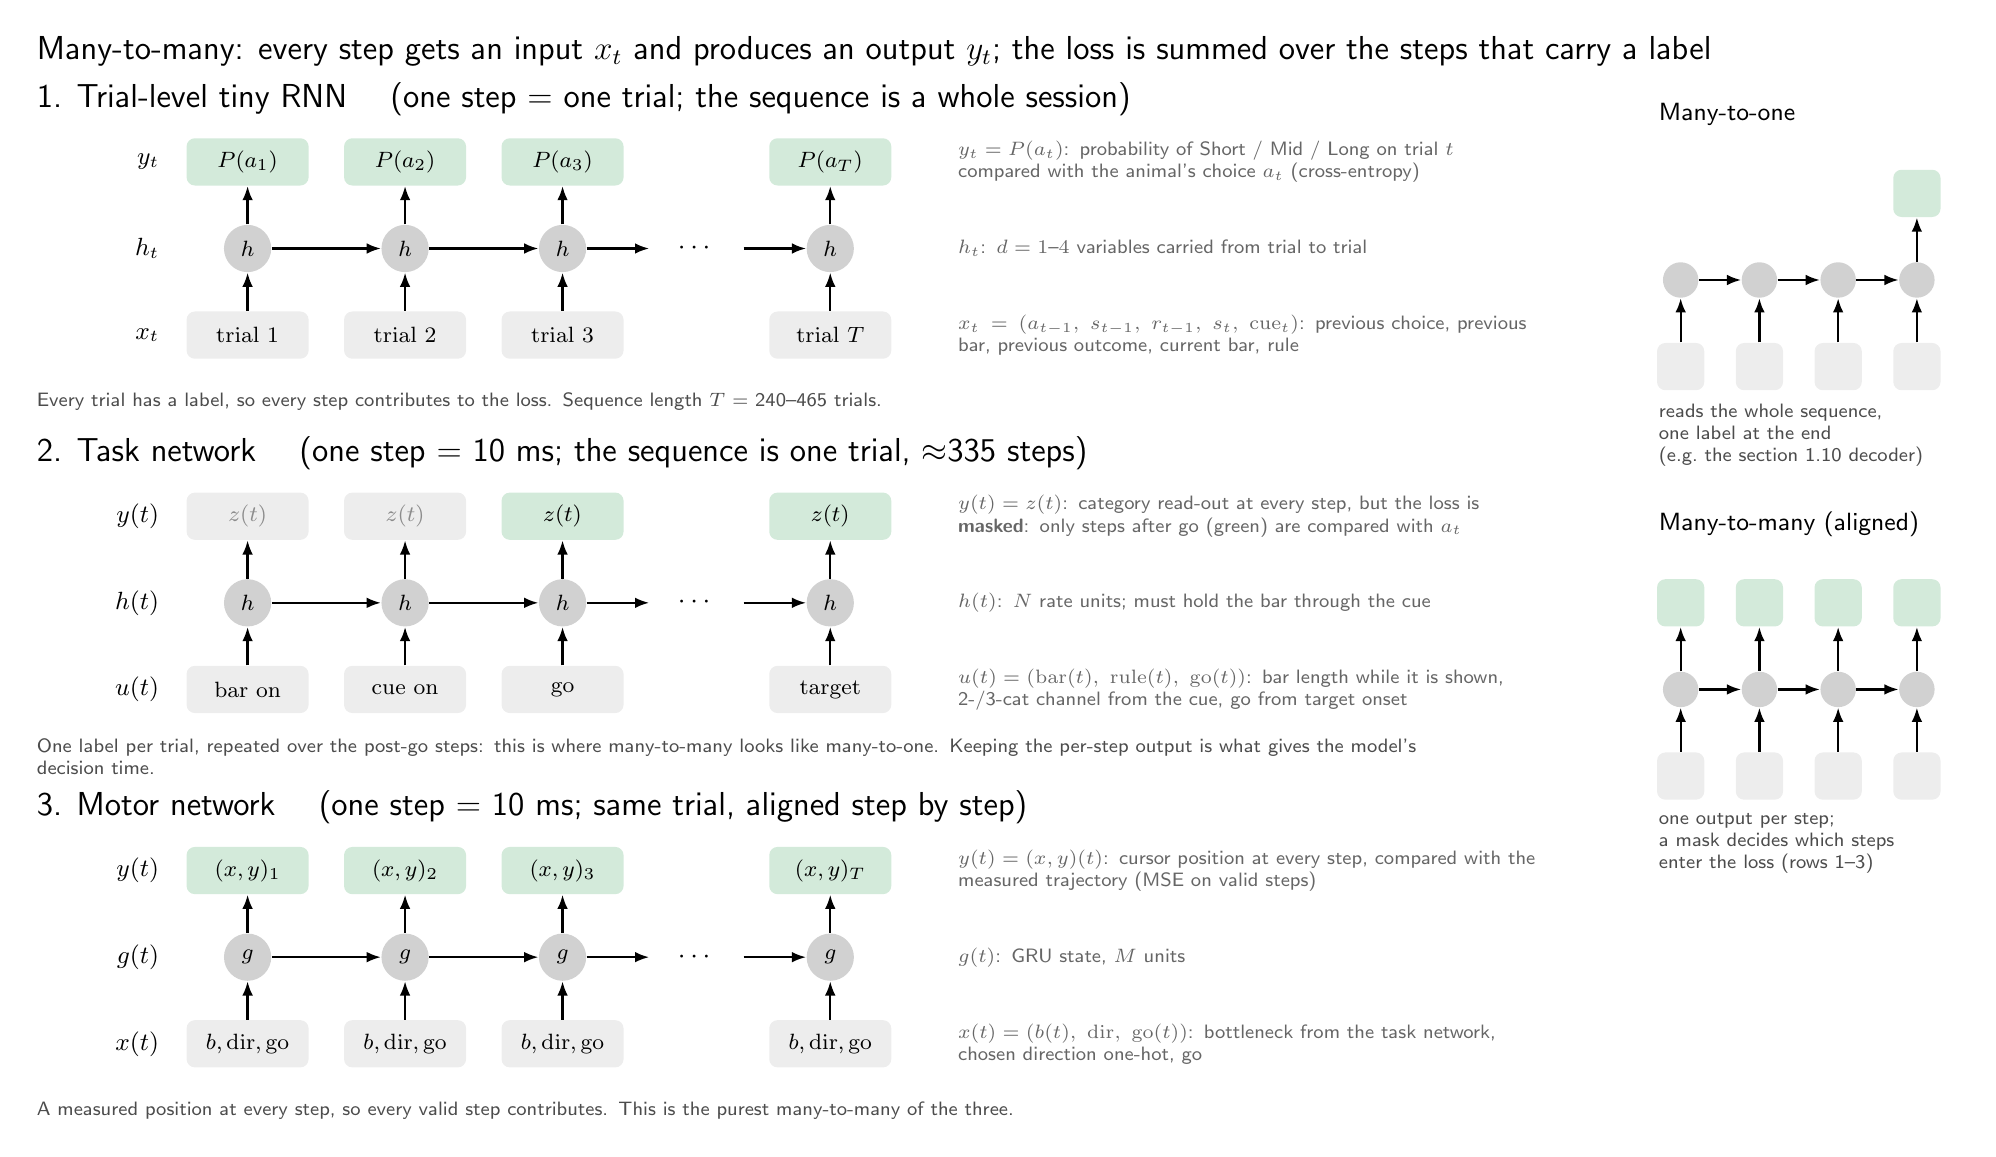
\begin{tikzpicture}[ctpanel,
  xin/.style={rounded corners=3pt, fill=black!7, draw=none, minimum width=1.55cm, minimum height=0.6cm, font=\footnotesize},
  yout/.style={rounded corners=3pt, fill=catMid!45, draw=none, minimum width=1.55cm, minimum height=0.6cm, font=\footnotesize},
  ynol/.style={rounded corners=3pt, fill=black!7, draw=none, minimum width=1.55cm, minimum height=0.6cm, font=\footnotesize, text=black!45},
  hid/.style={circle, fill=black!18, draw=none, minimum size=0.6cm, inner sep=0pt, font=\footnotesize},
  rec/.style={-{Latex[length=1.8mm]}, line width=0.8pt},
  lab/.style={font=\sffamily\small, anchor=east},
  note/.style={font=\sffamily\scriptsize, text=black!60, align=left, anchor=west, text width=7.6cm},
  wide/.style={text width=17.6cm},
  rowtitle/.style={font=\sffamily\large, anchor=west},
]

% one unrolled step: #1 x, #2 y, #3 input text, #4 output text, #5 style for y
\def\hlab{h}
\newcommand{\step}[5]{%
  \node[xin] (x#1) at (#2, 0)   {#3};
  \node[hid] (h#1) at (#2, 1.1) {$\hlab$};
  \node[#5]  (y#1) at (#2, 2.2) {#4};
  \draw[rec] (x#1) -- (h#1);
  \draw[rec] (h#1) -- (y#1);
}
\newcommand{\chain}[1]{\foreach \a/\b in {#1}{\draw[rec] (h\a) -- (h\b);}}

\node[font=\sffamily\large, anchor=west] at (-2.4,12.6)
  {Many-to-many: every step gets an input $x_t$ and produces an output $y_t$; the loss is summed over the steps that carry a label};

% =====================================================================
% Row 1: trial-level tiny RNN
% =====================================================================
\begin{scope}[yshift=9.0cm]
  \node[rowtitle] at (-2.4,3.0) {1. Trial-level tiny RNN \quad (one step = one trial; the sequence is a whole session)};
  \node[lab] at (-0.6,2.2) {$y_t$};
  \node[lab] at (-0.6,1.1) {$h_t$};
  \node[lab] at (-0.6,0)   {$x_t$};
  \step{a}{0.4}{trial 1}{$P(a_1)$}{yout}
  \step{b}{2.4}{trial 2}{$P(a_2)$}{yout}
  \step{c}{4.4}{trial 3}{$P(a_3)$}{yout}
  \node at (6.1,1.1) {$\cdots$};
  \step{d}{7.8}{trial $T$}{$P(a_T)$}{yout}
  \chain{a/b, b/c}
  \draw[rec] (hc) -- (5.5,1.1);
  \draw[rec] (6.7,1.1) -- (hd);
  \node[note] at (9.3,2.2) {$y_t = P(a_t)$: probability of Short / Mid / Long on trial $t$\\ compared with the animal's choice $a_t$ (cross-entropy)};
  \node[note] at (9.3,1.1) {$h_t$: $d = 1$--$4$ variables carried from trial to trial};
  \node[note] at (9.3,0)   {$x_t = (a_{t-1},\ s_{t-1},\ r_{t-1},\ s_t,\ \mathrm{cue}_t)$: previous choice, previous bar, previous outcome, current bar, rule};
  \node[note, wide, text=black!70] at (-2.4,-0.85) {Every trial has a label, so every step contributes to the loss. Sequence length $T$ = 240--465 trials.};
\end{scope}

% =====================================================================
% Row 2: within-trial task RNN
% =====================================================================
\begin{scope}[yshift=4.5cm]
  \node[rowtitle] at (-2.4,3.0) {2. Task network \quad (one step = 10 ms; the sequence is one trial, $\approx$335 steps)};
  \node[lab] at (-0.6,2.2) {$y(t)$};
  \node[lab] at (-0.6,1.1) {$h(t)$};
  \node[lab] at (-0.6,0)   {$u(t)$};
  \step{e}{0.4}{bar on}{$z(t)$}{ynol}
  \step{f}{2.4}{cue on}{$z(t)$}{ynol}
  \step{g}{4.4}{go}{$z(t)$}{yout}
  \node at (6.1,1.1) {$\cdots$};
  \step{h}{7.8}{target}{$z(t)$}{yout}
  \chain{e/f, f/g}
  \draw[rec] (hg) -- (5.5,1.1);
  \draw[rec] (6.7,1.1) -- (hh);
  \node[note] at (9.3,2.2) {$y(t) = z(t)$: category read-out at every step, but the loss is\\ \textbf{masked}: only steps after go (green) are compared with $a_t$};
  \node[note] at (9.3,1.1) {$h(t)$: $N$ rate units; must hold the bar through the cue};
  \node[note] at (9.3,0)   {$u(t) = (\mathrm{bar}(t),\ \mathrm{rule}(t),\ \mathrm{go}(t))$: bar length while it is shown,\\ 2-/3-cat channel from the cue, go from target onset};
  \node[note, wide, text=black!70] at (-2.4,-0.85) {One label per trial, repeated over the post-go steps: this is where many-to-many looks like many-to-one. Keeping the per-step output is what gives the model's decision time.};
\end{scope}

% =====================================================================
% Row 3: motor GRU
% =====================================================================
\begin{scope}[yshift=0cm]
  \def\hlab{g}
  \node[rowtitle] at (-2.4,3.0) {3. Motor network \quad (one step = 10 ms; same trial, aligned step by step)};
  \node[lab] at (-0.6,2.2) {$y(t)$};
  \node[lab] at (-0.6,1.1) {$g(t)$};
  \node[lab] at (-0.6,0)   {$x(t)$};
  \step{i}{0.4}{$b, \mathrm{dir}, \mathrm{go}$}{$(x,y)_1$}{yout}
  \step{j}{2.4}{$b, \mathrm{dir}, \mathrm{go}$}{$(x,y)_2$}{yout}
  \step{k}{4.4}{$b, \mathrm{dir}, \mathrm{go}$}{$(x,y)_3$}{yout}
  \node at (6.1,1.1) {$\cdots$};
  \step{l}{7.8}{$b, \mathrm{dir}, \mathrm{go}$}{$(x,y)_T$}{yout}
  \chain{i/j, j/k}
  \draw[rec] (hk) -- (5.5,1.1);
  \draw[rec] (6.7,1.1) -- (hl);
  \node[note] at (9.3,2.2) {$y(t) = (x, y)(t)$: cursor position at every step, compared with the\\ measured trajectory (MSE on valid steps)};
  \node[note] at (9.3,1.1) {$g(t)$: GRU state, $M$ units};
  \node[note] at (9.3,0)   {$x(t) = (b(t),\ \mathrm{dir},\ \mathrm{go}(t))$: bottleneck from the task network,\\ chosen direction one-hot, go};
  \node[note, wide, text=black!70] at (-2.4,-0.85) {A measured position at every step, so every valid step contributes. This is the purest many-to-many of the three.};
\end{scope}

% =====================================================================
% Right: topologies
% =====================================================================
\begin{scope}[xshift=18.6cm, yshift=8.6cm]
  \node[font=\sffamily\small, anchor=west] at (-0.4,3.2) {Many-to-one};
  \foreach \i/\x in {1/0, 2/1.0, 3/2.0, 4/3.0}{
    \node[xin, minimum width=0.6cm] (mx\i) at (\x,0) {};
    \node[hid, minimum size=0.45cm] (mh\i) at (\x,1.1) {};
    \draw[rec] (mx\i) -- (mh\i);
  }
  \foreach \a/\b in {1/2, 2/3, 3/4}{\draw[rec] (mh\a) -- (mh\b);}
  \node[yout, minimum width=0.6cm] (my) at (3.0,2.2) {};
  \draw[rec] (mh4) -- (my);
  \node[note, text=black!70, anchor=north west, text width=3.8cm] at (-0.4,-0.35) {reads the whole sequence,\\ one label at the end\\ (e.g.\ the section 1.10 decoder)};
\end{scope}

\begin{scope}[xshift=18.6cm, yshift=3.4cm]
  \node[font=\sffamily\small, anchor=west] at (-0.4,3.2) {Many-to-many (aligned)};
  \foreach \i/\x in {1/0, 2/1.0, 3/2.0, 4/3.0}{
    \node[xin, minimum width=0.6cm] (nx\i) at (\x,0) {};
    \node[hid, minimum size=0.45cm] (nh\i) at (\x,1.1) {};
    \node[yout, minimum width=0.6cm] (ny\i) at (\x,2.2) {};
    \draw[rec] (nx\i) -- (nh\i);
    \draw[rec] (nh\i) -- (ny\i);
  }
  \foreach \a/\b in {1/2, 2/3, 3/4}{\draw[rec] (nh\a) -- (nh\b);}
  \node[note, text=black!70, anchor=north west, text width=3.8cm] at (-0.4,-0.35) {one output per step;\\ a mask decides which steps\\ enter the loss (rows 1--3)};
\end{scope}

\end{tikzpicture}
\end{document}
